\documentclass[10pt,a5paper]{article}
\renewcommand{\baselinestretch}{1.0}
\usepackage{cite}
\usepackage[dvips]{graphicx}
\usepackage{psfrag}
\usepackage{color}
\usepackage[cmex10]{amsmath}
\usepackage{amsfonts}
\usepackage[font=footnotesize, captionskip=10pt]{subfig}
\usepackage{tikz}
\usepackage{flushend}
\usepackage{times}
\usepackage[margin=1.5cm]{geometry}
\pagestyle{empty}
\usepackage[slovak]{babel}
\usepackage[utf8]{inputenc}
\usepackage[T1]{fontenc}


\usepackage[]{algorithm2e}
\usepackage{listings}
 \usepackage{cuted}
\usepackage[export]{adjustbox}
\usepackage{mathtools}

\usepackage{lipsum}
\usepackage{verbatim}
\usepackage{transparent}
\usepackage{framed}
\usepackage{xcolor}

\usepackage{multirow}
\usepackage{colortbl}

\usepackage{lipsum}
\usepackage{mathtools}
\usepackage{cuted}
\usepackage{hyperref}

\hyphenation{net-works}
\newtheorem{remark}{Remark}

\begin{document}

\title{Umelá inteligancia v počítačových hrách}
\author{Michal Chovanec,
michal.chovanec@fri.uniza.sk}
\date{}
\maketitle
\thispagestyle{empty}

Kurz je určený pre tých, ktorí už vedia programovať a chcú sa posunúť ďalej.
Programovať sa bude v Pythone v OS Linux (notebooky si netreba priniesť).
Na niekoľkých príkladoch si ukážeme ako je možné pomocou odmeňovania naučiť bota
hrať takmer ľubovolnú hru. Bot sa sám naučí čo je najlepšie robiť vo rôznych situáciach.
Zdrojáky na stiahnutie nájdeš na \url{https://github.com/michalnand/deep\_learning\_systems/tree/master/rl\_exercises}
\\
\\



        \begin{minipage}{0.5\textwidth}

            \noindent {\bf Čo sa naučíš:}
            \begin{itemize}
            \item {\bf Naprogramuješ} jednoduchú hru
            \item Dozvieš sa čo je to {\bf deep learning}
            \item Natrénuješ {\bf neurónovú sieť}
            \item Vytvoríš bota, ktorý {\bf sa sám učí}
            \end{itemize}

            \noindent {\bf Obsah:}
            \begin{enumerate}
            \item Tvorba herného mechanizmu
            \item Grafické rozhranie s OpenGL a prvý bot ktorý sa sám učí
            \item Bot s hlbokou neurónovou sieťou
            \item Súťaž kto natrénuje lepšieho bota
            \end{enumerate}

        \end{minipage}
        \begin{minipage}{0.5\textwidth}
             \vspace{-2ex}
              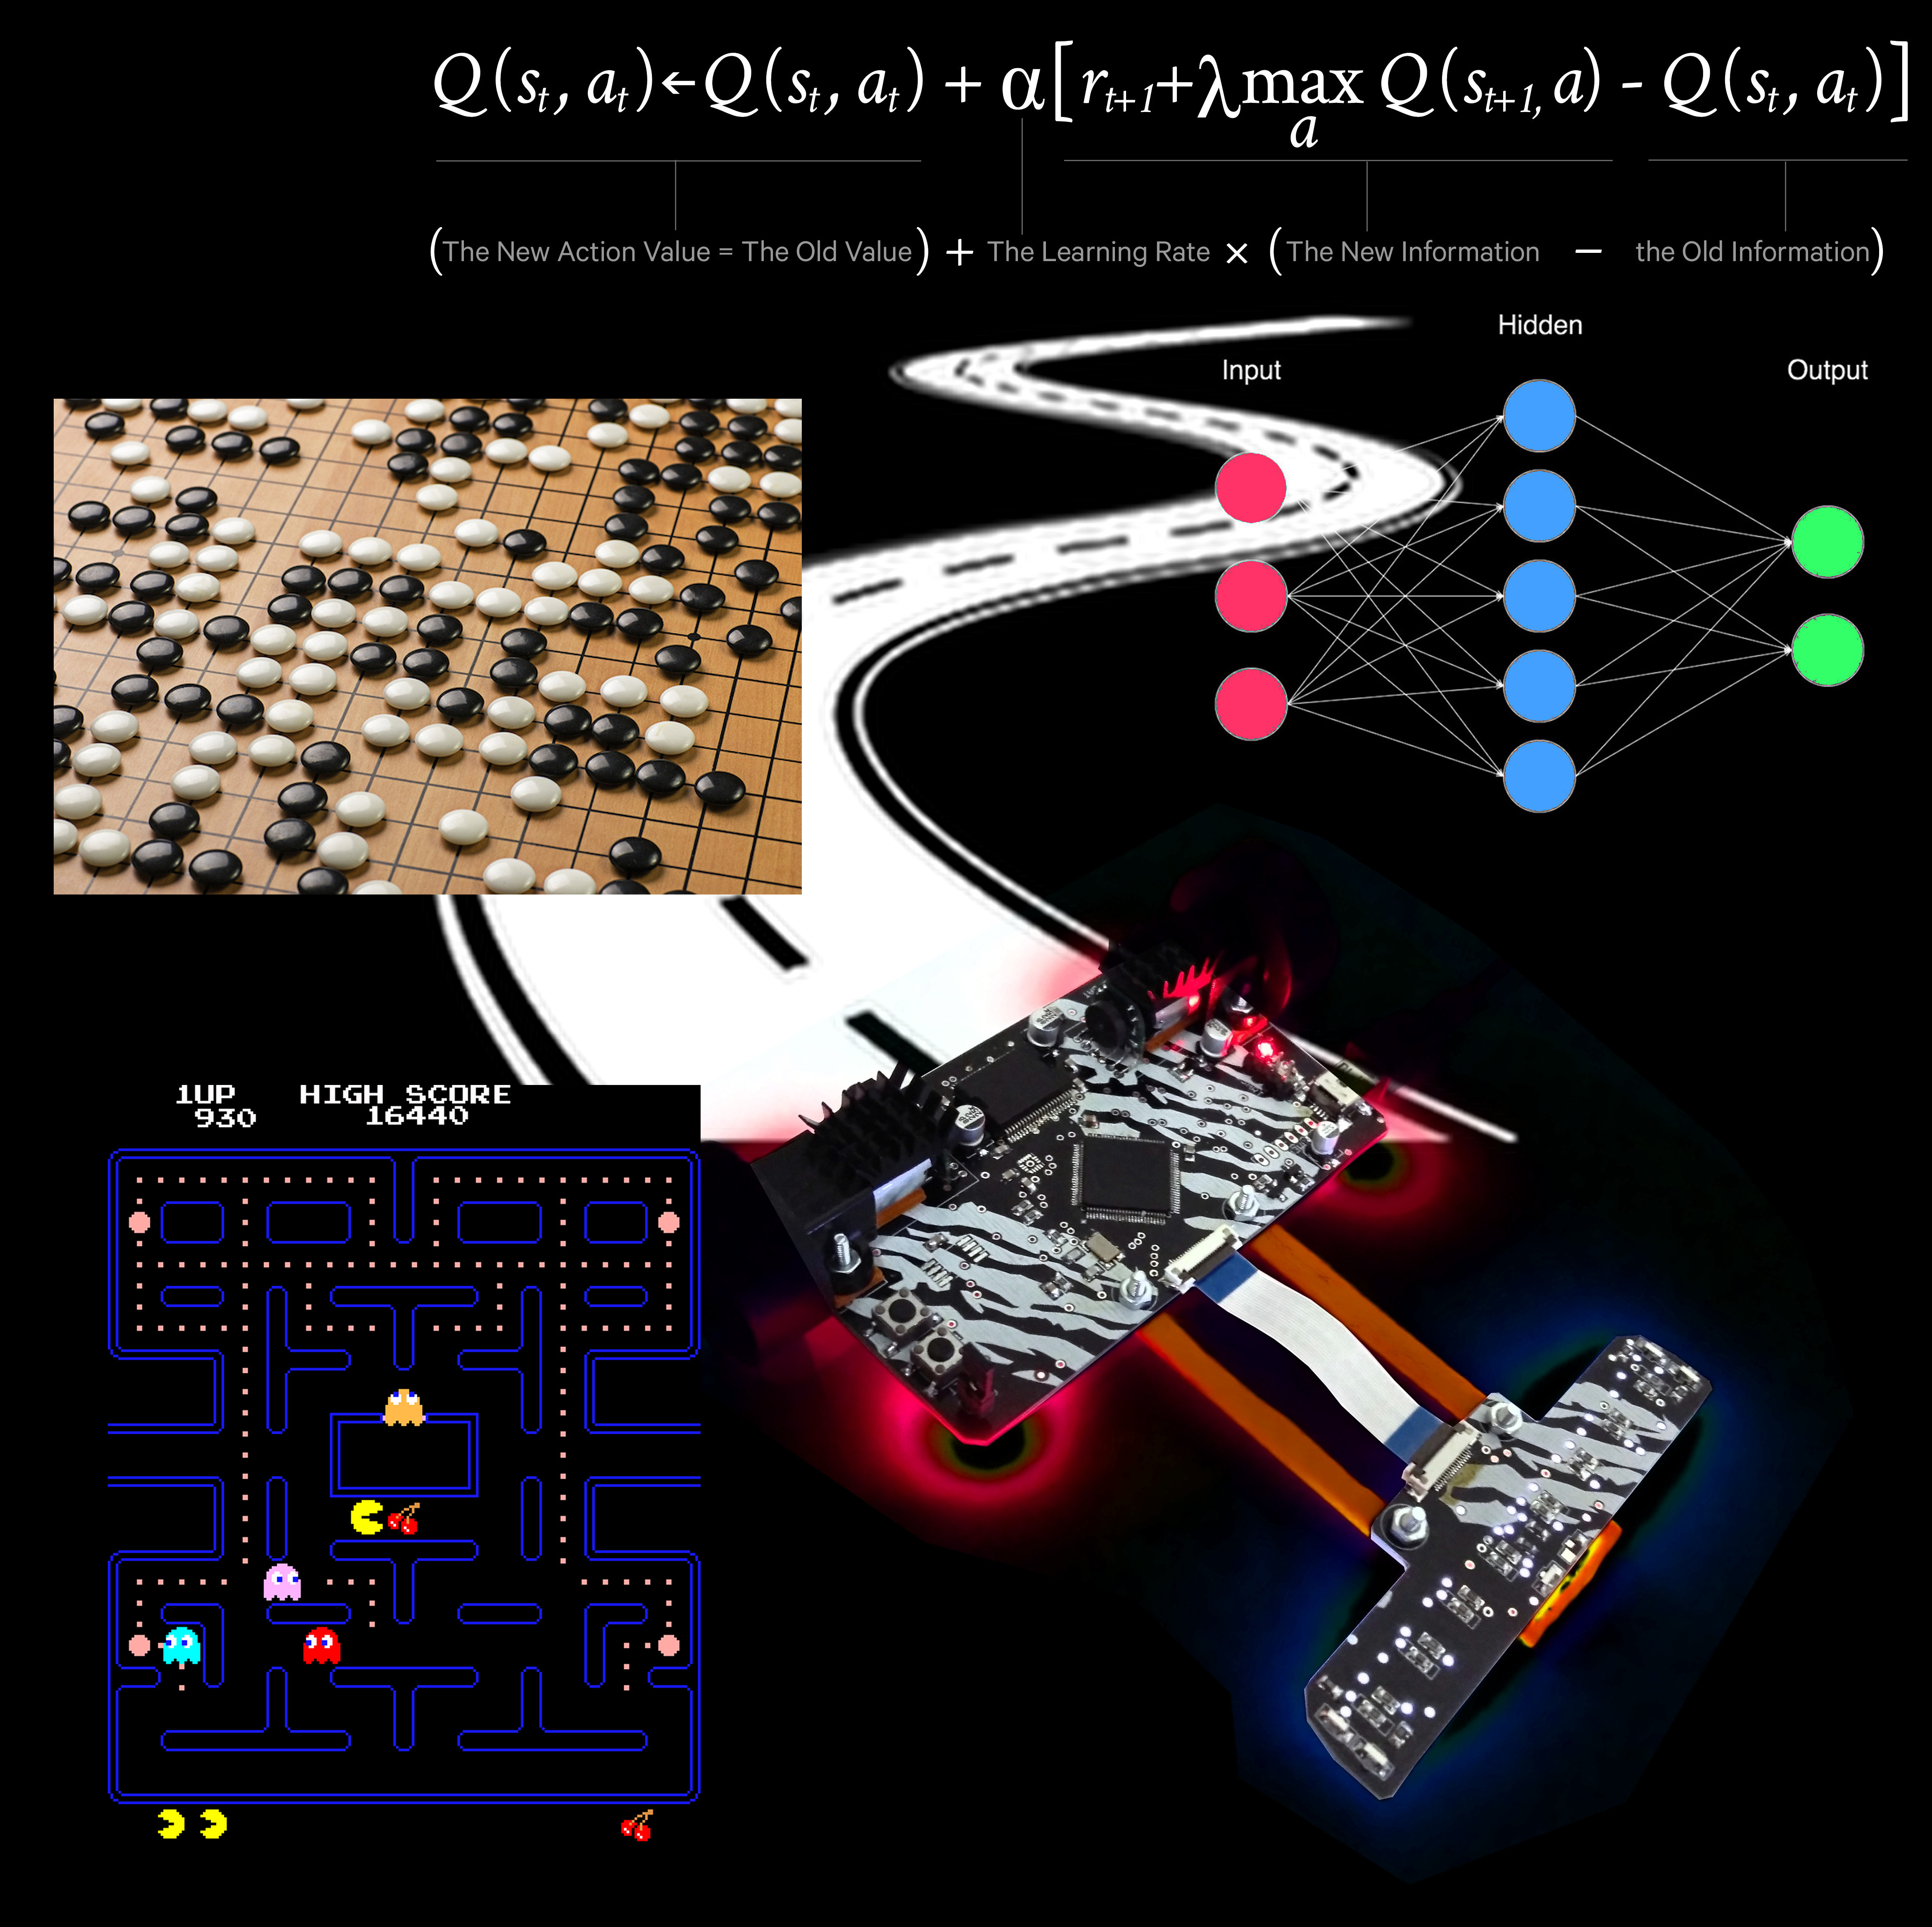
\includegraphics[scale=0.04]{../../pictures/rl_square_2.jpg}

        \end{minipage}





\end{document}
